\section{Insights from the features}
To understand the phenomenon of user engagement with the mico video content, we extract the above listed features from the sampled frames and extracted audio tracks of the videos. The motivation behind this excercise was to find peculiar discriminators amongst these features with respect to engagement. The following section describes some of the saliant differences between the high engagement and low engagement micro videos. To analyse the features, we sampled the videos twice every second and represented the whole 6 second long video as a series of 12 static frames. This sampling rate is not too low to miss any considerable frame transitions, neither is too high to include a lot of mid transition frames. 

\subsection{Faces engage us}
For analysing this feature, we run the viola jones face detector for profile and frontal faces on every frame of the selected videos. Once sampled videos were processed for presence of faces, we analysed their prevalence seperately for the high engagement videos sampeld from the POP12K dataset and the low engagement videos sampled from the ALL120K dataset. The figure \ref{fig:Face_CDF} shows the CDF of the percentage of face frames relative to total frames in a micro video. It is notable to see that highly engaging videos, tend to have a higher percentage of face frames. This shows a deeper behaviour of users, a tendency to be engaged to human faces. 

\begin{figure}[!htb]
\centering
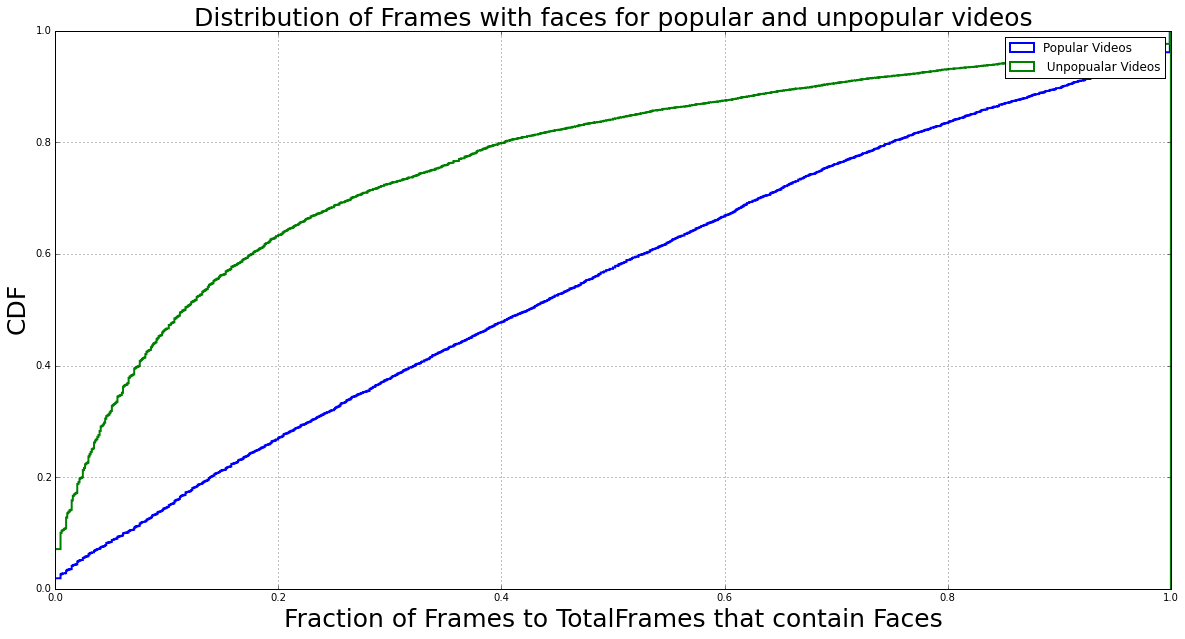
\includegraphics[width=\columnwidth]{plots/FaceCDF}
\caption{\textsl{ CDF for popular and unpopular videos. The CDF signifies the cumulative distribution of percentages of face containing frames in a vine video. The observation here is popular videos tend to have higher percentages than unpopular videos}}
\label{fig:Face_CDF}
\end{figure}

\subsection{ Too short to make an impact ?}
Image sentiments extracted using Sentibank framework are basically a good measure to understand the sentiment of the producer of the image. Because these detectors were trained on static images downloaded from flicker they do a good job of understanding some sort of an abstract sentiment from an image. We wanted to explore the time signatures of these abstract frame sentiments for micro videos. . To do this  we processed all the sampled frames using the Sentibank deeplearning framework to estimate sentiment of each frame on a scale of 0 to 5. The detailed reasoning and description of this sentiment scale can be found in\cite{jou2015visual}. 
We now had a \textit{N} x 12 matrix of sentiment time signatures for \textit{N} videos. In our case \textit{N} is 12,000 micro videos, 6000 from POP12K and 6000 from ALL120K dataset. To understand if there are any patterns in the sentiment transitions across the videos, the frame transition matrix of dimension 12000x12 was clusterd using K means clustering algorithm (cite). But to find the right amount of clusters we used the elbow method (cite). In the elbow method, k-means is iteratively run over the complete dataset for different values of K ranging from 1 to a resonably high maximum. We run till K = 10. At each step the sum of squred distance is calculated for every cluster between the cluster centroid and all the other vectors which are member of the cluster. 
\begin{equation}
SSD = \sum_{i =1}^{K = 10} \sum_{X \in{N}}{dist(X,c_i)}^2
\end{equation}

We then plot the array of SSDs and look for and change in rate of decrease of SSDs, also called as the elbow point, on the graph. The value of K for which this point occurs has the most tight grouping of points in the 12 dimentional space when clustered in K clusters. From Fig \ref{fig:Elbow_method} , this point is found to be at K = 4 in our case. 

\begin{figure}[!htb]
\centering
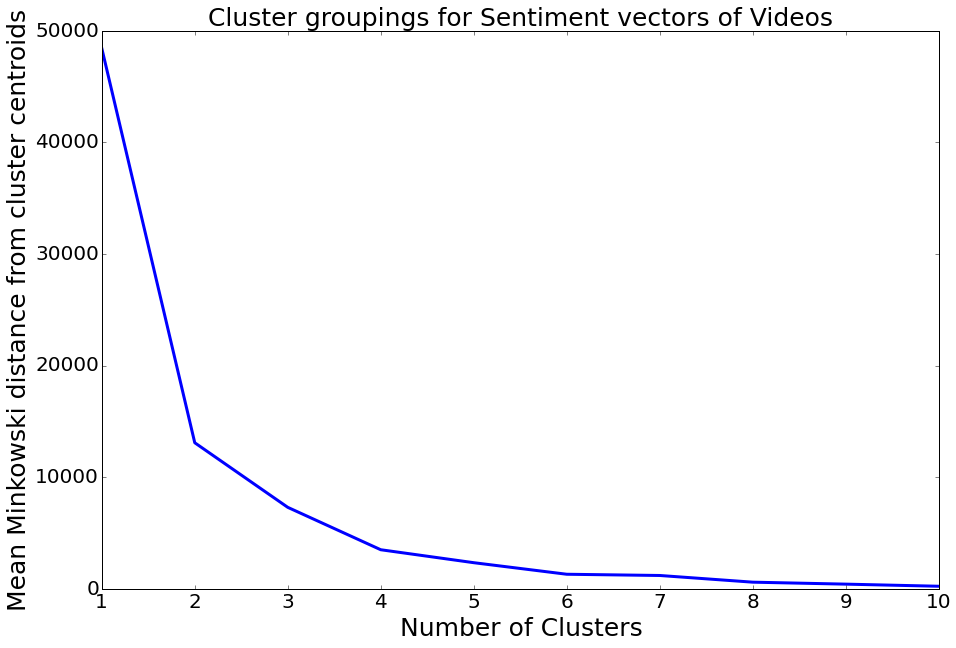
\includegraphics[width=\columnwidth]{plots/grouping_graph_clusters}
\caption{\textsl{The Sentiment transition matrix was analysed for existence of clusters, using the elbow points method for mean Euclidean distance (Minkowski distance for p = 2). We found that the best grouping exists at K=4 }}
\label{fig:Elbow_method}
\end{figure}

Using this elbow point, we cluster the Matrix and look for salient trends in transition, by plotting the values of centroids of each cluster. The Fig \ref{fig:Clusters} shows that despite being seperated in the sentiment space, the values of sentiments remain constant for a given cluster. The paper does not explore the fundamental reason behind this, but it is a peculiar behaviour. One possible hypothesis behind this could be that 6 seconds is too short a period for the creators of Micro videos, to project any kind of percievable and impactful change in frame sentiments. 

\begin{figure}[!htb]
\centering
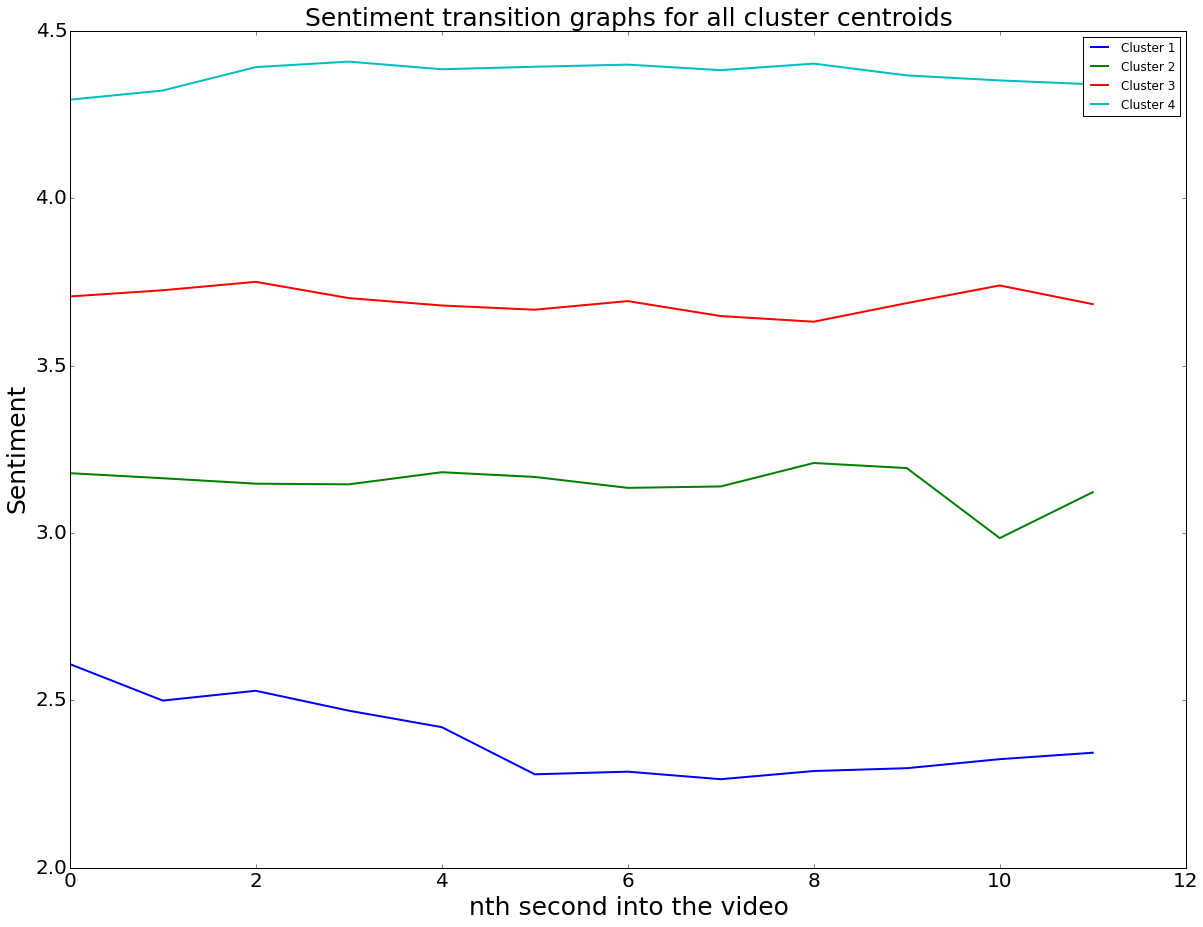
\includegraphics[width=\columnwidth]{plots/4_cluster_senti}
\caption{\textsl{ Plot of frame sentiment vectors, of the 4 centroids of the clusters found. The vine videos  tend to have a constant sentiment structure at 4 distinct sentiment levels }}
\label{fig:Clusters}
\end{figure}


\subsection{First impression lasts}
The whole idea of a user engaging with a micro video on Vine, involves the process of scrolling past videos and then keeping a video in focus so as to trigger the auto looping mechanism described in introduction. This whole user experience makes engagement highly influenced by how far the user plays the video. To understand the effect of frame sentiments in different parts if vidoe over this user behavious, we plotted a simple histogram of the frequency of occance of maximum or minumum frame sentiments against the thirds of video. A trend that was evident from this was that the probability of coming across the most positive or the most negative sentiment in a micro video is the highest in the first one third of the video and progresively decays (Fig \ref{fig:Senti_Thirds}

\begin{figure}[!htb]
\centering
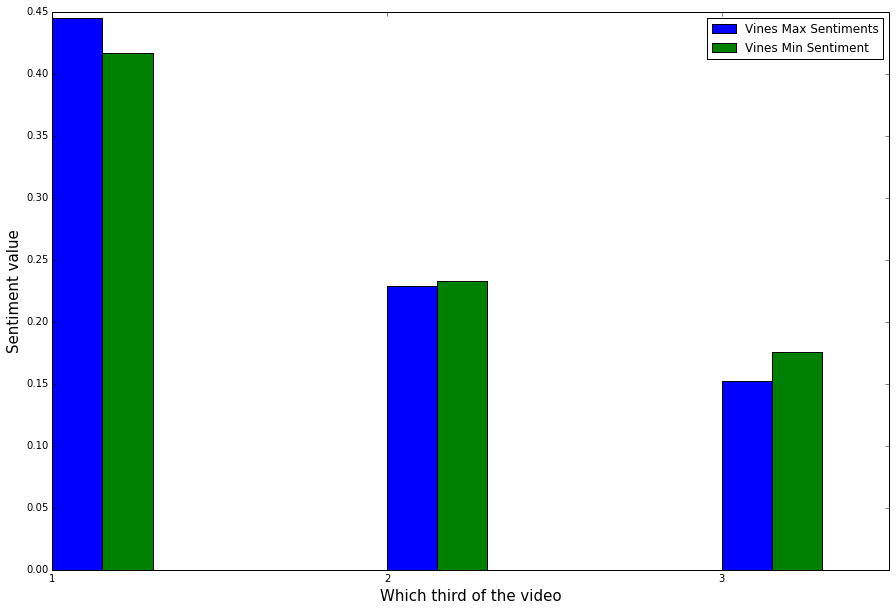
\includegraphics[width=\columnwidth]{plots/SentimentsThirds}
\caption{\textsl{ Frequency of occurance of maximum or minimum sentiment. For this graph, the video is considered in thirds, and the frequency of occurance of both max and min frame sentiments is plotted. }}
\label{fig:Senti_Thirds}
\end{figure} 

We repeated a similar process for aesthetic features. There too, we found a similar trend of the first one third of video having the best overall aesthetic quality (\ref{fig:Aesthetic_trends}

\begin{figure}[!htb]
\centering
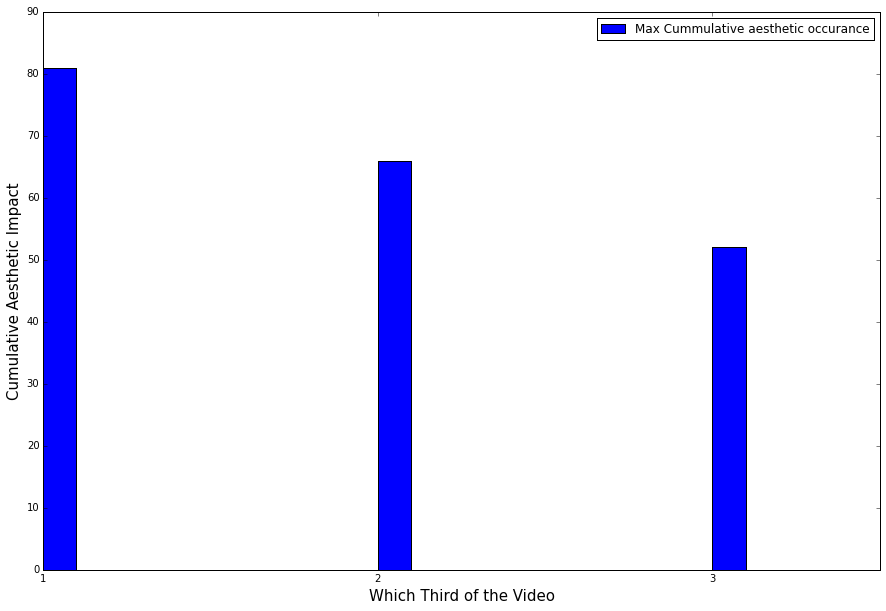
\includegraphics[width=\columnwidth]{plots/cumulativeAestheticImpact}
\caption{\textsl{ Plot of cumulative aesthetic impact of each third of the video. For this plot the videos were sampled at one frame a second, and aesthetic features were calculated at every second. Finally the features were  }}
\label{fig:Aesthetic_trends}
\end{figure} 

These two trends say something about the producer behaviour. \ns{How should I close this insight? What should I draw any conclusion from this or let the classifier experiment talk about it ?}

\subsection{Quality matters, but not that much}

Aesthetics are important part of any social media analysis. They are going to play a part in garnering user engaagement. But how much? 
To comment about this question, we needed a comparision of overall aesthetics of micro videos with some sort of a gold standard for highy aesthetic images. Hence we compare the aesthetic features of frames sampled from both high engagement micro videos and low engagement videos, with images taken from the dataset sourced from photo.net \cite{datta2008algorithmic}. These images were rated for aesthetic appeal for the research involved and these ratings are also used while selecting the images for our comparison. We only choose images with median ratings of 6 or above on aesthetic scale of 0 to 7.  The table \ref{aesthetic_table} shows the comparison of means and medians of several of these aesthetic features compared to the highly aesthetic dataset. From the table it is quite evident that Aesthetics in micro videos matter, but they are no way close to what one can call aesthetically pleasing frames. 

\begin{table}
\caption{List of Aesthetic parameters computed for highly rated aesthetic images, Popular videos and unpopular videos. Most parameters have no bias towards either popular or unpopular videos}

\resizebox{\linewidth}{!}{%
\begin{tabular}{|l|*{11}{c|}}
  \hline
   Parameter & \multicolumn{2}{|c|}{Aesthetic Images}  &  \multicolumn{2}{|c|}{Popular Vines} & \multicolumn{2}{|c|}{Unpopular Vines} \\ \hline
   \_ & Mean&Median&Mean&Median&Mean&Median\\ \hline
   \ Color Contrast & 51.05 & 30.22 & 29.88 &16.43 & 20.23  & 8.83  \\ \hline
   \ Intensity Balance & 0.11 & 0.08 & 0.16 & 0.13 & 0.17 & 0.14 \\ \hline
   \ Luo Simplicity & 0.009 & 0.005 & 0.013 & 0.012 & 0.015  & 0.014  \\ \hline
   \ Sharp pixel proportion & 0.103 & 0.098 & 0.090 & 0.085 & 0.089  & 0.081  \\ \hline
   \ Image Saturation & 0.943 & 0.974 & 0.672 & 0.678 & 0.615  & 0.646  \\ \hline
   \ Avg. Brightness & 0.148 & 0.141 & 0.137 & 0.130 & 0.139  & 0.124  \\ \hline
   \ Rule of Thirds & 0.879 & 0.899 & 0.883 & 0.883 & 0.878  &0.882  \\ \hline
   \ ROI Proportion & 0.316 & 0.089 & 0.175 & 0.112 & 0.165  & 0.110  \\ \hline
\end{tabular}}
\label{aesthetic_table}
\end{table}
